\documentclass[11pt]{article}
\usepackage{amsmath,graphicx,color,epsfig,physics}
%\usepackage{pstricks}
\usepackage{float}
\usepackage{subfigure}
\usepackage{slashed}
\usepackage{color}
\usepackage{multirow}
\usepackage{feynmp}
\usepackage[top=1in, bottom=1in, left=1.2in, right=1.2in]{geometry}
\begin{document}
\title{Particle physics HW2}
\author{Yang Ma}

\maketitle


\section{ }
For Gaussian distribution
\begin{eqnarray}
  P(x)=\frac{1}{\sqrt{2 \pi \sigma^2}}\exp{-\frac{(x-\mu)^2}{2\sigma^2}},
\end{eqnarray}
one have
\begin{eqnarray}
  \int_{-\infty}^{\infty} d x P(x) &=& \frac{1}{\sqrt{2 \pi \sigma^2}} \int_{-\infty}^{\infty} \exp{-\frac{(x-\mu)^2}{2\sigma^2}} d (x-\mu)\nonumber \\
  &=&\frac{\sqrt{2 \pi \sigma^2}}{\sqrt{2 \pi \sigma^2}} =1.
\end{eqnarray}

\section{ }
\begin{eqnarray}
  <x> &=&\int_{-\infty}^{\infty} x d x P(x) = \frac{1}{\sqrt{2 \pi \sigma^2}} \int_{-\infty}^{\infty} x \exp{-\frac{(x-\mu)^2}{2\sigma^2}} dx \nonumber \\
  &=& \frac{1}{\sqrt{2 \pi \sigma^2}} \left [ \int_{-\infty}^{\infty} (x-\mu) \exp{-\frac{(x-\mu)^2}{2\sigma^2}} dx +  \int_{-\infty}^{\infty} \mu \exp{-\frac{(x-\mu)^2}{2\sigma^2}} dx \right ] \nonumber \\
  &=& 0+ \mu =\mu
\end{eqnarray}

\section{ }
By setting $\sigma\to1$,$\mu \to 5$, we can plot $P(x)$ as a function of $x$ in Fig.\ref{fig.2_3}. The range $\mu -\sigma < x < \mu +\sigma$ now become $4 < x < 6$. One straightforward way to calculate this numerical integral is to pick up several points of $x$, and we pick up 20 points with step $0.1$ from $x=4$ to $x=6$. The area is then $\sum_x P(x) \delta s\approx 0.704$, which is clsoed to $67\%$.
\begin{figure}[htb]
  \centering
  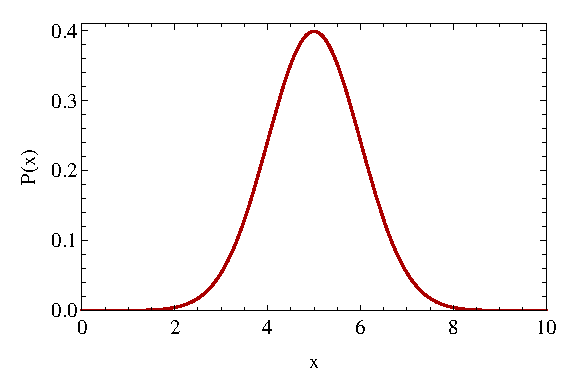
\includegraphics[width=8cm]{2_3.eps}
  \caption{$P(x)$ as a function of $x$.\label{fig.2_3}}
\end{figure}


\section{ }
With the pion mass $m_{\pi^{\pm}}$=140MeV, we have $\gamma=E/m_{\pi^{\pm}}=10$, and
\begin{eqnarray}
l=c \tau \gamma \beta = 3 \times 10^8 \times 2.6\times 10^{-8} \times 10 = 78 {\rm m}.
\end{eqnarray}
This can also be obtained using the mean decay length
\begin{eqnarray}
  l=c \tau \gamma \beta = 1 \times 780 {\rm cm} \times 10 \times 1=78 {\rm m}.
\end{eqnarray}

\section{ }
Now we also have $\gamma=10$ for muon. Using its mean decah length $l=6.6 \times 10^6$cm, we have
\begin{eqnarray}
  l=c \tau \gamma \beta= 6600 {\rm m}.
\end{eqnarray}

\section{ }
For 22kton water, one can obtain the number of proton
\begin{eqnarray}
  \frac {22 \times 10^6 \times 10 \times 6.022 \times 10^{23}}{18 \times 10^-3}=7.4 \times 10^{33}.
\end{eqnarray}
The number of particles is a function of time $t$ and the lifetime of the given particle $\tau$,
\begin{eqnarray}
  N(t)=N_0 e^{-\frac{t}{\tau}}.
\end{eqnarray}
Then we have the number of decay events
\begin{eqnarray}
  N_0 (1-e^{-\frac{t}{\tau}}) \approx N_0 \frac{t}{\tau}=\frac {7.4 \times 10^{33} \times 20}{8 \times 10^{33}}=18.5.
\end{eqnarray}

\section{ }
With the transfromation
\begin{eqnarray}
  z \to z'=e^{i \theta} z,
\end{eqnarray}
we see
\begin{eqnarray}
  |z'|^2=|e^{i \theta} z|^2=1\times |z|^2=|z|^2.
\end{eqnarray}

\section{ }
\begin{eqnarray}
  e^{i \theta}&=&\sum^\infty_{n=0}(i \theta)^n/n! \nonumber \\
  &=&\sum_{m=0}^{m=\infty}  (i\theta )^{2m}/{2m}! + (i \theta )^{2m+1}/(2m+1)! \\
  &=&\sum_{m=0}^{m=\infty} \theta ^{2m}/{2m}!+i \sum_{m=0}^{n=\infty} \theta^{2m+1}/(2m+1)!\\
  &=&\cos \theta + i \sin \theta.
\end{eqnarray}

\section{ }
With $z \to z'= e^{i \theta} z$, we have 
\begin{eqnarray}
  z'&=&  e^{i \theta} (x+iy) =(\cos \theta +i \sin \theta) (x+iy)\\
  &=& (\cos \theta x-\sin \theta y)+i (\sin \theta x \cos \theta y) \\
  &=& x'+iy',
\end{eqnarray}
which can be summarized as
\begin{eqnarray}
  \begin{pmatrix}
    x\\y 
  \end{pmatrix} \rightarrow
  \begin{pmatrix}
    x'\\y'
  \end{pmatrix} = 
  \begin{pmatrix}
    \cos \theta & -\sin \theta\\
    \sin \theta&\cos \theta
  \end{pmatrix}
  \begin{pmatrix}
    x\\y
  \end{pmatrix}
\end{eqnarray}

\section {}
With
\begin{eqnarray}
  O=
  \begin{pmatrix}
    \cos \theta & -\sin \theta\\
    \sin \theta&\cos \theta
  \end{pmatrix},
\end{eqnarray}
and
\begin{eqnarray}
  O^T=
  \begin{pmatrix}
    \cos \theta & \sin \theta\\
    -\sin \theta&\cos \theta
  \end{pmatrix},
\end{eqnarray}
we see
\begin{eqnarray}
  O O^T=
  \begin{pmatrix}
    \cos^2 \theta + \sin^2 \theta &0 \\
    0 & \cos^2 \theta + \sin^2 \theta
  \end{pmatrix}
  = 1.
\end{eqnarray}

\section{ }

\begin{eqnarray}
  J=
  \begin{pmatrix}
    o & -i\\
    i & 0
  \end{pmatrix},
\end{eqnarray}
Define $U(\theta)=I e^{i J \theta}=\sum_{n=0}^\infty=\frac{(ij\theta)^n}{n!}$, and we have
\begin{eqnarray}
U_{11}&=&\sum_{m=0}^{m=\infty} \theta ^{2m}/{2m}!=\cos \theta,\nonumber \\
U_{12}&=&\sum_{m=0}^{m=\infty} \theta ^{2m+1}/(2m+1)!=\sin \theta,\nonumber \\
U_{21}&=&-\sum_{m=0}^{m=\infty} \theta ^{2m+1}/(2m+1)!=-\sin \theta,\nonumber \\
U_{22}&=&\sum_{m=0}^{m=\infty} \theta ^{2m}/{2m}!=\cos \theta.
\end{eqnarray}
We see that $J$ covers all U(1) transfromation.

\section{ }
\begin{itemize}
  \item For $U(\theta)=e^{i \theta}$, we have
  \begin{eqnarray}
    U(\theta_1) U(\theta_2) &=&e^{i \theta_1} e^{i \theta_2} =e^{i (\theta_1+\theta_2)}=U(\theta_1+\theta_2) \nonumber \\
    U(\theta_1) (U(\theta_2) U(\theta_3)) &=& e^{i (\theta_1+\theta_2+\theta_3)}= (U(\theta_1) U(\theta_2)) U(\theta_3).
  \end{eqnarray}
  Note that $U(\theta)=I$ when $\theta=0$, then we have
  \begin{eqnarray}
    U(\theta) U(0)=U(\theta) I= U(\theta) = U(0) U(\theta),
  \end{eqnarray}
  and
  \begin{eqnarray}
    U(\theta) U(- \theta)=U (0).
  \end{eqnarray}
  \item For
  \begin{eqnarray}
    O=
    \begin{pmatrix}
      \cos \theta & -\sin \theta\\
      \sin \theta&\cos \theta
    \end{pmatrix},
  \end{eqnarray}
  we have
  \begin{eqnarray}
    O(\theta_1) O(\theta_2) &=&
    \begin{pmatrix}
      \cos \theta_1 \cos \theta_2-\sin \theta_1 \sin\theta_2 & -\cos\theta_1 \sin\theta_2-\sin\theta_1 \cos\theta_2\\
      \sin\theta_1 \cos\theta_2+\sin \theta_2\cos\theta_1 &
      \cos\theta_1\cos \theta_2-\sin\theta_1\sin\theta_2
    \end{pmatrix}\\
    &=&
    \begin{pmatrix}
      \cos(\theta_1+\theta_2)&-\sin_(\theta_1+\theta_2) \\
      \sin_(\theta_1+\theta_2) & \cos(\theta_1+\theta_2)
    \end{pmatrix}=O(\theta_1+\theta_2).
  \end{eqnarray}
  Then it is easy to have
  \begin{eqnarray}
    O(\theta_1) (O(\theta_2) O(\theta_3))&=&O(\theta_1)O(\theta_2+\theta_3)= O(\theta_1+\theta_2+\theta_3)\\
    &=& O(\theta_1+ \theta_2)O(\theta_3)=(O(\theta_1) O(\theta_2)) O(\theta_3).
  \end{eqnarray}
  Note that $O(\theta)=I$ when $\theta=0$, then we have
  \begin{eqnarray}
    O(\theta) O(0)=O(\theta) I= O(\theta) = O(0) O(\theta),
  \end{eqnarray}
  and
  \begin{eqnarray}
    O(\theta) O(- \theta)=O (0).
  \end{eqnarray}
  
  \item For the inverse transfromations, we just replace $\theta$ with $\theta$ and above discussion will still be valid.

\end{itemize}

\section{ }
For $SU(2)$, we have
\begin{eqnarray}
  U(\theta)=
  \begin{pmatrix}
    \cos \frac{\theta}{2} & i\sin \frac{\theta}{2} \\
    i\sin \frac{\theta}{2} & \cos \frac{\theta}{2}
  \end{pmatrix}
\end{eqnarray}
and
\begin{eqnarray}
  z'= U(\theta) z = 
  \begin{pmatrix}
    \cos \frac{\theta}{2} z_1 + i\sin \frac{\theta}{2} z_2 \\
    i\sin \frac{\theta}{2} z_1+ \cos \frac{\theta}{2} z-2
  \end{pmatrix},
\end{eqnarray}
so we have
\begin{eqnarray}
  |z_1'|^2+|z_2'|^2=&&(x_1 \cos \frac{\theta}{2}-y_2 \sin \frac{\theta}{2})^2+(x_2 \sin \frac{\theta}{2} + y_1\cos \frac{\theta}{2} )^2 \nonumber \\
  &&+ (x_2 \cos \frac{\theta}{2}-y_1 \sin \frac{\theta}{2})^2+(x_1 \sin \frac{\theta}{2} + y_2\cos \frac{\theta}{2} )^2\\
  =&& x_1^2+x_2^2+y_1^2+y_2^2=|z_1|^2+|z_2|^2
\end{eqnarray}

\end{document}